\documentclass[10pt]{beamer}
\usepackage{lmodern}
\usepackage[utf8]{vietnam}
\usepackage{amsmath}
\usepackage{listings}
\usepackage{xcolor}
\usepackage{multicol}
\usefonttheme{structurebold}
\usetheme{Rochester}

\usepackage[backend=biber]{biblatex}

\definecolor{codegreen}{rgb}{0,0.6,0}
\definecolor{codegray}{rgb}{0.5,0.5,0.5}
\definecolor{codepurple}{rgb}{0.58,0,0.82}
\definecolor{backcolour}{rgb}{0.95,0.95,0.92}

\lstdefinestyle{mystyle}{
    backgroundcolor=\color{backcolour},   
    commentstyle=\color{codegreen},
    keywordstyle=\color{magenta},
    numberstyle=\tiny\color{codegray},
    stringstyle=\color{codepurple},
    basicstyle=\ttfamily\footnotesize,
    breakatwhitespace=false,         
    breaklines=true,                 
    captionpos=b,                    
    keepspaces=true,                 
    numbers=left,                    
    numbersep=5pt,                  
    showspaces=false,                
    showstringspaces=false,
    showtabs=false,                  
    tabsize=2
}

\lstset{style=mystyle}


\addbibresource{presentation.bib}

\setbeamertemplate{footline}[frame number]

\setbeamertemplate{navigation symbols}{\insertlogo}

\begin{document}
\author{Đoàn Thu Ngân, Trần Hoàng Quân, Huỳnh Tấn Thọ, Sử Nhật Đăng, Phan Đặng Diễm Uyên}
\title{Tính hiệu quả của Phương pháp Đơn hình}
\subtitle{Tìm hiểu hiệu năng của Phương pháp Đơn hình khi giải một bài toán QHTT có kích thước cố định.}
\logo{
\includegraphics[scale=.2]{img/fithcmuslogo.png}}
\institute{VNUHCM - University of Science}
%\date{Spring 2022}
\subject{CSC10104 - Linear Programming}

\setbeamercovered{transparent}
\setbeamertemplate{navigation symbols}{}

\begin{frame}[plain]
\maketitle
\end{frame}

\begin{frame}
\frametitle{Mục lục}
\tableofcontents
\end{frame}

\section{Ước lượng hiệu năng thuật toán}
\begin{frame}{Ước lượng hiệu năng thuật toán}
Xét các bài toán có cùng kích thước cố định, việc ước lượng hiệu năng có thể được chia thành 2 loại:
\begin{itemize}
\item Trường hợp xấu nhất: Tính toán chi phí cần thiết để giải bài toán \textbf{phức tạp nhất} trong số các bài toán đã cho.
\item Trường hợp trung bình: Tính toán chi phí \textbf{trung bình} khi giải các bài toán có cùng kích thước.
\end{itemize}
\end{frame}

\begin{frame}{Ước lượng hiệu năng thuật toán (cont.)}
\begin{multicols}{2}
Để đưa ra một ước lượng cho trường hợp xấu nhất
\begin{itemize}
\item Ta tìm một chi phí \textit{cận trên}.
\item Đưa ra một ví dụ chứng minh thuật toán đạt được chi phí cận này.
\end{itemize}
\columnbreak
\begin{figure}
\centering
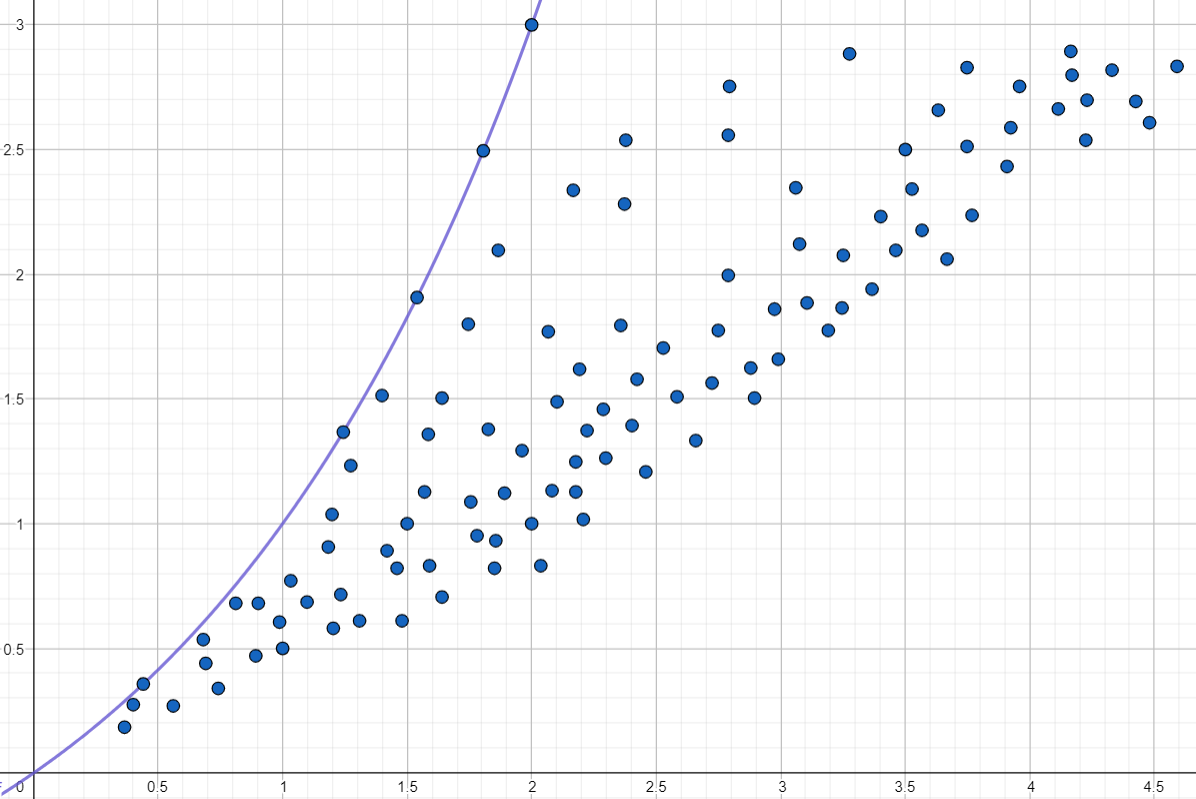
\includegraphics[width=\linewidth]{img/worst-case.png}
\caption{Đồ thị biểu diễn chi phí thuật toán trong trường hợp xấu nhất}
\end{figure}
\end{multicols}
\end{frame}

\begin{frame}{Ước lượng hiệu năng thuật toán (cont.)}
\begin{multicols}{2}
Để ước lượng  trường hợp trung bình, ta cần một \textit{mô hình ngẫu nhiên}\footnote{stochastic model} từ các bài toán quy hoạch tuyến tính được tạo \textit{ngẫu nhiên}. Từ đây, ta phát sinh 2 vấn đề:
\begin{itemize}
\item Ta không rõ làm thế nào để tạo ra một mô hình như vậy.
\item Sau khi có mô hình, ta phải đánh giá chi phí cho \textbf{mọi} bài toán của mô hình trên.
\end{itemize}
\columnbreak
\begin{figure}
\centering
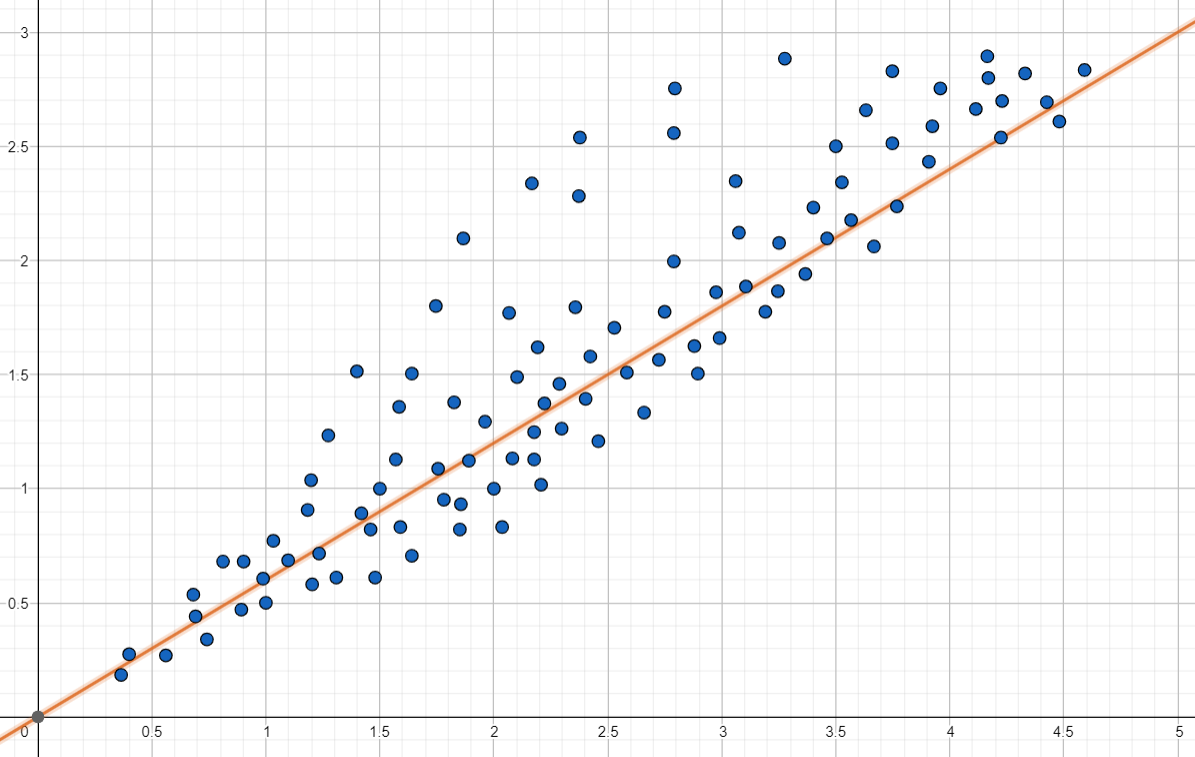
\includegraphics[width=\linewidth]{img/average-case.png}
\caption{Đồ thị biểu diễn chi phí thuật toán trong trường hợp trung bình}
\end{figure}
\end{multicols}
\end{frame}

\begin{frame}{Ước lượng hiệu năng thuật toán (cont.)}
\begin{itemize}
\item Dễ thấy, trường hợp xấu nhất nhìn chung dễ ước lượng hơn so với trường hợp trung bình.
\item Tuy nhiên, trường hợp xấu nhất không sát với các bài toán gặp phải trong thực tế.
\end{itemize}
\end{frame}

\begin{frame}{Ước lượng kích thước bài toán}
Đầu tiên, làm cách nào để xác định kích thước bài toán?\\
\begin{itemize}
\item Hai tham số được nhắc đến một cách tự nhiên là $m$ - số ràng buộc và $n$ - số biến.
\item Tổng số phần tử trong dữ liệu bài toán là $m\times n$.
\item Kích thước bài toán = $m\times n$.
\end{itemize}
\end{frame}

\begin{frame}{Ước lượng kích thước bài toán (cont.)}
Nếu bài toán có nhiều hoặc hầu hết các phần tử bằng 0?
\begin{itemize}
\item Dữ liệu đầu vào có nhiều số 0 cải thiện hiệu năng của bài toán.
\item Kích thước bài toán = tổng số phần tử khác 0 trong dữ liệu.
\end{itemize}
\end{frame}

\begin{frame}{Ước lượng kích thước bài toán (cont.)}
Trong thực tế
\begin{itemize}
\item Tốc độ tính toán của con người (hoặc máy tính có độ chính xác vô hạn) khi nhân hai số khác nhau phụ thuộc vào kiểu dữ liệu của hai số
\item Ví dụ: 23 $\times$ 7 sẽ nhanh hơn 23,453.2352 $\times$ 86,833.245643
\end{itemize}
$\rightarrow$ Cách tính tốt hơn: \textbf{số lượng bit} cần thiết để lưu trữ dữ liệu bài toán trên máy tính - ký hiệu \textit{L}.
\end{frame}

\begin{frame}{Ước lượng kích thước bài toán (cont.)}
Tuy nhiên, kết quả \textit{L} còn mơ hồ, không thể xác định rõ là
\begin{itemize}
\item Số lượng bit đầu vào cần thiết để chỉ rõ các hệ số ràng buộc, hệ số hàm mục tiêu, kết quả vế phải khác 0.
\item Số lượng bit trong dữ liệu gốc + Số lượng bit trong mô tả bài toán.
\end{itemize}
$\rightarrow$ Ta chỉ tập trung vào hai tham số $m$ và $n$ khi mô tả kích thước bài toán.
\end{frame}


\section{Ước lượng chi phí tính toán}
\begin{frame}{Ước lượng chi phí tính toán}
Thứ hai, làm thế nào để xác định chi phí để giải một bài toán?\\
Câu trả lời tốt nhất là \textit{số giây} mà máy tính cần để giải bài toán
\begin{itemize}
\item Tuy nhiên, không phải mọi người đều dùng chung một kiểu máy tính.
\item Các công nghệ dành cho máy tính thay đổi nhanh chóng.
\item Việc đề xuất dùng một mẫu máy tính làm chuẩn chung cho việc đánh giá thuật toán là không khả thi.
\end{itemize}
\end{frame}

\begin{frame}{Ước lượng chi phí tính toán (cont.)}
Một giải pháp thay thế
\begin{itemize}
\item Thuật toán nói chung là các quá trình lặp đi lặp lại. Do đó, ta có thể sử dụng \textit{số lần lặp} làm thước đo.
\item Số lần lặp của một thuật toán \textbf{không phụ thuộc} vào tốc độ tính toán máy tính.
\item Thời gian để giải một bài toán = số lần lặp cần để giải bài toán $\times$ thời gian cần để máy tính thực hiện một lần lặp.
\end{itemize}
\end{frame}

\begin{frame}{Ước lượng chi phí tính toán (cont.)}  
\begin{itemize}
\item Với các thuật toán khác nhau trong cùng một lớp thuật toán chung, thời gian cần để thực hiện một lần lặp có thể giống nhau giữa các thuật toán.\\
$\rightarrow$ Việc chọn số lần lặp làm thước đo là phù hợp
\item Tuy nhiên, khi ta muốn so sánh hai thuật toán hoàn toàn khác nhau, việc chọn số lần lặp để ước lượng chi phí là không có ý nghĩa.
\end{itemize}
\end{frame}

\begin{frame}{Ước lượng chi phí tính toán (cont.)}  
\begin{itemize}
\item  Hiện tại, chúng ta sẽ ước lượng chi phí để giải một bài toán quy hoạch tuyến tính bằng cách đếm số lần lặp (hay chính là số phần tử xoay - pivot) cần thiết để giải nó.
\end{itemize}
\end{frame}

\section{Đánh giá trường hợp xấu nhất}
\begin{frame}{Nhắc lại phương pháp đơn hình}
Cho bài toán QHTT có $n$ biến, $m$ ràng buộc.
Hàm mục tiêu
$$
f = \sum_{j=1}^{n}c_jx_j \rightarrow \max\ (\min)
$$
Hệ các ràng buộc
\begin{equation*}
\begin{aligned}
x_{Bi} + \sum_{j \notin B}a_{ij}x_{Bj} &= b_i, &i = \overline{1, m}\\
x_j &\leq 0, &j = \overline{1, n}
\end{aligned}
\end{equation*}
Với $b \leq 0$, bài toán có phương án cơ bản ban đầu
\begin{equation*}
\begin{aligned}
x_{B_i}^0 &= b_i, &i = \overline{1, m}\\
x_j^0 &= 0, &j \notin B
\end{aligned}
\end{equation*}
\end{frame}

\begin{frame}{Nhắc lại Phương pháp đơn hình (cont.)}
\textbf{Bước 1:} Lập bảng đơn hình xuất phát
\begin{table}[H]
\centering
\begin{tabular}{|c|c|c|c|c|c|c|}
\hline
Cơ sở & Hệ số & Phương án & $c_1$ & $c_2$ & $...$ & $c_n$\\
\hline
$x_1$ & $c_1$ & $b_1$ & $a_{11}$ & $a_{12}$ & $...$ & $a_{1n}$ \\
$x_2$ & $c_2$ & $b_2$ & $a_{21}$ & $a_{22}$ & $...$ & $a_{2n}$ \\
$\vdots$ & $\vdots$ & $\vdots$ & $\vdots$ & $\vdots$ & $\vdots$ & $\vdots$\\
$x_m$ & $c_m$ & $b_m$ & $a_{m1}$ & $a_{m2}$ & $...$ & $a_{mn}$\\
\hline
$f$ & & $\Delta_0$ & $\Delta_1$ & $\Delta_2$ & $...$ & $\Delta_n$ \\
\hline
\end{tabular}
\end{table}
trong đó
$$
\Delta_0 = \sum^{m}_{i=1}c_{i}.b_i,\ \Delta_i = \sum^{m}_{i=1}c_i.a_{ij} - c_j
$$

\end{frame}

\begin{frame}{Nhắc lại Phương pháp đơn hình (cont.)}
\textbf{Bước 2:} Biện luận
\begin{itemize}
\item Trong bài toán tìm \textbf{min}, thuật toán dừng khi tất cả $\Delta \leq 0$. Nếu còn $\Delta > 0$, ta chọn số lớn nhất, và trên cột tương ứng, ta chọn phần tử xoay $a_{ij}$ theo tiêu chí: nó là số dương và tỷ số $\dfrac{b_{i}}{a_{ij}}$ là nhỏ nhất.
\item Trong bài toán tìm \textbf{max}, thuật toán dừng khi tất cả $\Delta \geq 0$. Nếu còn $\Delta < 0$, ta chọn số âm nhỏ nhất, và trên cột tương ứng, ta chọn phần tử xoay $a_{ij}$ theo tiêu chí: nó là số dương và tỷ số $\dfrac{b_{i}}{a_{ij}}$ là nhỏ nhất.
\end{itemize}
Ta chọn được phần tử xoay và thực hiện phép khử để tìm phương án mới.
\end{frame}

\begin{frame}{Đánh giá trường hợp xấu nhất}
Một vài nhận xét:
\begin{itemize}
\item Số phương án chấp nhận được tối đa có thể chọn là $\displaystyle \binom{n + m}{n}$.
\item Trong trường hợp xấu nhất, $n + m$ đạt giá trị lớn nhất khi $m = n$.
\end{itemize}
Khi đó số phương án chấp nhận được tối đa có thể chọn:
$$
\displaystyle \binom{n + n}{n} = \binom{2n}{n}
$$
Ta cũng có thể ước lượng một chặn trên và chặn dưới của thuật toán\cite{Vanderbei2020}:
$$
\frac{2^{2n}}{2n} \leq \binom{2n}{n} \leq 2^{2n} \ (n \in \mathbb{N^+})
$$
\end{frame}

\begin{frame}{Đánh giá trường hợp xấu nhất (cont.) - Chứng minh}
\begin{theorem}[Xấp xỉ Stirling\cite{weisstein}]
$$
\displaystyle
n! \operatorname*{\sim}_{n\to\infty} \sqrt{2\pi n}\left(\frac{n}{e}\right)^n
$$
\end{theorem}
Khai triển $\displaystyle \binom{2n}{n} = \frac{(2n)!}{(n!)^2}$\footnote{$\binom{n}{k} = \frac{n!}{(n - k)!k!}$}. Ta cũng có các xấp xỉ sau:
\begin{itemize}
\item $\displaystyle (2n)! \operatorname*{\sim}_{n\to\infty} 2\sqrt{\pi n} \left(\frac{2n}{e}\right)^{2n}$ 
\item $\displaystyle (n!)^2 \operatorname*{\sim}_{n\to\infty} 2\pi n \left(\frac{n}{e}\right)^{2n}$ 
\end{itemize}
Qua đó, $\displaystyle \binom{2n}{n} \operatorname*{\sim}_{n\to\infty} \frac{2\sqrt{\pi n} \left(\frac{2n}{e}\right)^{2n}}{2\pi n \left(\frac{n}{e}\right)^{2n}} =  \frac{2^{2n}}{\sqrt{\pi n}}$
\end{frame}

\begin{frame}{Đánh giá trường hợp xấu nhất (cont.) - Chứng minh}
\begin{proof}
Gọi
$$
\displaystyle
L = \frac{\frac{2^{2n}}{2n}}{\frac{2^{2n}}{\sqrt{\pi n}}} = \frac{2^{2n}\sqrt{\pi n}}{2^{2n} 2n} = \frac{\sqrt{\pi}}{2\sqrt{n}} < 1,\ \forall n \in \mathbb{N^+}
$$
Do $L < 1$, ta có thể kết luận $\frac{2^{2n}}{2n} \leq \frac{2^{2n}}{\sqrt{\pi n}},\ \forall n \in \mathbb{N^+}
$. Khi đó
$$
\displaystyle
\frac{2^{2n}}{2n} \leq \frac{2^{2n}}{\sqrt{\pi n}} \leq 2^{2n} \iff \frac{2^{2n}}{2n} \leq \binom{2n}{n} \leq 2^{2n}
$$
\end{proof}
Trong trường hợp xấu nhất, thuật toán có độ phức tạp thuộc nhóm $\mathcal{O}(2^{2n})$. $2^{2n}$ \textbf{rất lớn} dù $n$ không lớn lắm. (e.g $n = 25$, $2^{50} = 1.1259\times 10^{15}$)
\end{frame}

\begin{frame}{Đánh giá trường hợp xấu nhất (cont.) - Ví dụ}
Năm 1972, V. Klee and G.J. Minty\cite{klee1970good} đề xuất bài toán Minty-Klee, theo đó phương pháp đơn hình cần ít nhất $2^n - 1$ lần lặp để giải:
$$
\sum_{j = 1}^{n} 2^{n - j} x_j \rightarrow \max
$$
các ràng buộc
\begin{equation*}
\begin{aligned}
2\sum_{j = 1}^{i - 1} 2^{i - j}x_j + x_i &\leq 100^{i - 1} & (i = 1, 2, .., n)\\
x_j &\geq 0 & (j = 1, 2, .., n)
\end{aligned}
\end{equation*}
Theo đó 3 ràng buộc đầu tiên
$$
\left\{
\begin{array}{lll}
x_1 &\leq 1\\
4x_1 + x_2 &\leq 10^2\\
8x_1 + 4x_2 + x_3 &\leq 10^4
\end{array}
\right.
$$
\end{frame}

\begin{frame}{Đánh giá trường hợp xấu nhất (cont.) - Ví dụ}
Dễ thấy đây chỉ là tập các cận trên của mỗi biến:
$$
\begin{array}{lll}
0 \leq x_1 &\leq 1\\
0 \leq x_2 &\leq 10^2\\
0 \leq x_3 &\leq 10^4
\end{array}
$$
Do đó, tập các ràng buộc trở thành tập các cận trên (upper-bound set), biến miền ràng buộc trên không gian $n$ chiều thành một siêu lập phương:
$$
\begin{array}{lll}
0 \leq x_1 &\leq 1\\
0 \leq x_2 &\leq 100\\
&\vdots\\
0 \leq x_n &\leq 100^{n - 1}
\end{array}
$$
\end{frame}

\begin{frame}{Đánh giá trường hợp xấu nhất (cont.) - Ví dụ}
Miền chấp thuận của bài toán Klee-Minty còn được gọi là Siêu lập phương\footnote{Siêu lập phương $n$ chiều có $2^n$ đỉnh\cite{10945-3852}} Klee-Minty.
\begin{figure}
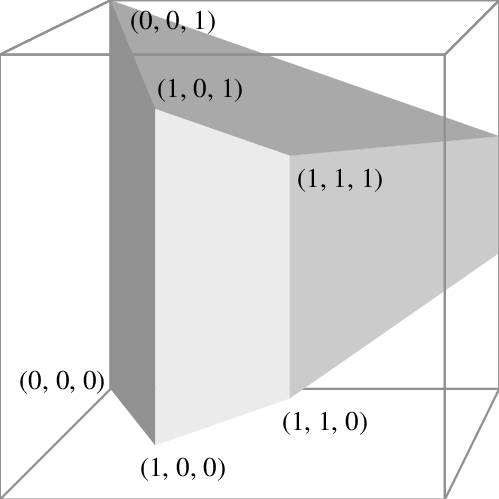
\includegraphics[scale=.15]{img/klee-minty-cube.png}
\caption{Ví dụ cho Siêu lập phương Klee-Minty với $n = 3$ và $\epsilon = \frac{1}{3}$}
\end{figure}
Phương pháp đơn hình sẽ xuất phát từ 1 đỉnh, đi qua tất cả các đỉnh trước khi tìm ra phương án tối ưu.
\end{frame}

\begin{frame}{Đánh giá trường hợp xấu nhất (cont.) - Ví dụ}
Đặt $\beta_i = 100^{i - 1}$. Bài toán Minty-Klee có dạng tổng quát:
$$
\sum_{j = 1}^n 2^{n - j}x_j - \frac{1}{2}\sum_{j = 1}^n 2^{n - j}\beta_j \rightarrow \max
$$
các ràng buộc
$$
\begin{aligned}
2\sum_{j = 1}^{i - 1} 2^{i - j}x_j + x_i &\leq \sum_{j = 1}^{i - 1}2^{i - j}\beta_j + \beta_i\ &(i = 1, 2, .., n)\\
x_j &\geq 0 &(j = 1, 2, .., n)
\end{aligned}
$$
\end{frame}

\begin{frame}{Đánh giá trường hợp xấu nhất (cont.) - Ví dụ}
Với $n = 3$, bài toán được phát biểu như sau:
$$
4x_1 + 2x_2 + x_3 - 2\beta_1 - \beta_2 - \frac{1}{2}\beta_3 \rightarrow \max
$$
Các ràng buộc:
$$
\left\{
\begin{array}{lll}
x_1 &\leq \beta_1\\
4x_1 + x_2 &\leq 2\beta_1 + \beta_2\\
8x_1 + 4x_2 + x_3 &\leq 4\beta_1 + 2\beta_2 + \beta_3
\end{array}
\right.
$$
Ta thêm biến để được các đẳng thức:
$$
\left\{
\begin{array}{lll}
x_1 & + \ x_4 & = \beta_1\\
4x_1 + x_2 & + \ x_5 & = 2\beta_1 + \beta_2\\
8x_1 + 4x_2 + x_3 & + \ x_6 & = 4\beta_1 + 2\beta_2 + \beta_3\\
x_4, \ x_5, \ x_6 & &\geq 0
\end{array}
\right.
$$
Cơ sở: $(x_4, x_5, x_6)$
\end{frame}

\begin{frame}{Đánh giá trường hợp xấu nhất (cont.) - Ví dụ}
Bảng đơn hình xuất phát:
\begin{table}[H]
\centering
\begin{tabular}{|c|c|c|c|c|c|c|c|c|}
\hline
CS & HS & PA & 4 & 2 & 1 & 0 & 0 & 0 \\
\hline
$x_4$ & 0 & $\beta_1$ & 1 & 0 & 0 & 1 & 0 & 0 \\
$x_5$ & 0 & $2\beta_1 + \beta_2$ & 4 & 1 & 0 & 0 & 1 & 0 \\
$x_6$ & 0 & $4\beta_1 + 2\beta_2 + \beta_3$ & 8 & 4 & 1 & 0 & 0 & 1 \\
\hline
\multicolumn{2}{|c|}{max}
& 0 & -4 & -2 & -1 & 0 & 0 & 0 \\
\hline
\end{tabular}
\end{table}
\begin{itemize}
\item Tồn tại 3 cột ứng với $\Delta < 0$, ta chọn cột có $\Delta = -4$  
\item So sánh: $\dfrac{\beta_1}{1} < \dfrac{2\beta_1 + \beta_2}{4} < \dfrac{4\beta_1 + 2\beta_2 + \beta_3}{8}$ nên ta chọn dòng 1  
\item $x_4$ ra, $x_1$ vào
\end{itemize}
\end{frame}

\begin{frame}{Đánh giá trường hợp xấu nhất (cont.) - Ví dụ}
Lần lặp thứ 1:
\begin{table}[H]
\centering
\begin{tabular}{|c|c|c|c|c|c|c|c|c|}
\hline
CS & HS & PA & 4 & 2 & 1 & 0 & 0 & 0 \\
\hline
$x_1$ & 4 & $\beta_1$ & 1 & 0 & 0 & 1 & 0 & 0 \\
$x_5$ & 0 & $-2\beta_1 + \beta_2$ & 0 & 1 & 0 & -4 & 1 & 0 \\
$x_6$ & 0 & $-4\beta_1 + 2\beta_2 + \beta_3$ & 0 & 4 & 1 & -8 & 0 & 1 \\
\hline
\multicolumn{2}{|c|}{max}
& $4\beta_1$ & 0 & -2 & -1 & 4 & 0 & 0 \\
\hline
\end{tabular}
\end{table}
\begin{itemize}
\item Tồn tại 2 cột ứng với $\Delta < 0$, ta chọn cột có $\Delta = -2$
\item So sánh: $\dfrac{-2\beta_1 + \beta_2}{1} < \dfrac{-4\beta_1 + 2\beta_2 + \beta_3}{4}$ nên ta chọn dòng 2
\item $x_5$ ra, $x_2$ vào
\end{itemize}
\end{frame}

\begin{frame}{Đánh giá trường hợp xấu nhất (cont.) - Ví dụ}
Lần lặp thứ 2:
\begin{table}[H]
\centering
\begin{tabular}{|c|c|c|c|c|c|c|c|c|}
\hline
CS & HS & PA & 4 & 2 & 1 & 0 & 0 & 0 \\
\hline
$x_1$ & 4 & $\beta_1$ & 1 & 0 & 0 & 1 & 0 & 0 \\
$x_2$ & 2 & $-2\beta_1 + \beta_2$ & 0 & 1 & 0 & -4 & 1 & 0 \\
$x_6$ & 0 & $4\beta_1 - 2\beta_2 + \beta_3$ & 0 & 0 & 1 & 8 & -4 & 1 \\
\hline
\multicolumn{2}{|c|}{max}
& $2\beta_2$ & 0 & 0 & -1 & -4 & 2 & 0 \\
\hline
\end{tabular}
\end{table}
\begin{itemize}
\item Tồn tại 2 cột ứng với $\Delta < 0$, ta chọn cột có $\Delta = -4$
\item So sánh: $\dfrac{\beta_1}{1} < \dfrac{4\beta_1 - 2\beta_2 + \beta_3}{8}$ nên ta chọn dòng 1
\item $x_1$ ra, $x_4$ vào
\end{itemize}
\end{frame}

\begin{frame}{Đánh giá trường hợp xấu nhất (cont.) - Ví dụ}
Lần lặp thứ 3:
\begin{table}[H]
\centering
\begin{tabular}{|c|c|c|c|c|c|c|c|c|}
\hline
CS & HS & PA & 4 & 2 & 1 & 0 & 0 & 0 \\
\hline
$x_4$ & 0 & $\beta_1$ & 1 & 0 & 0 & 1 & 0 & 0 \\
$x_2$ & 2 & $2\beta_1 + \beta_2$ & 4 & 1 & 0 & 0 & 1 & 0 \\
$x_6$ & 0 & $-4\beta_1 - 2\beta_2 + \beta_3$ & -8 & 0 & 1 & 0 & -4 & 1 \\
\hline
\multicolumn{2}{|c|}{max}
& $4\beta_1 + 2\beta_2$ & 4 & 0 & -1 & 0 & 2 & 0 \\
\hline
\end{tabular}
\end{table}
\begin{itemize}
\item Tồn tại 1 cột ứng với $\Delta < 0$, ta chọn cột $\Delta = -1$
\item $x_6$ ra, $x_3$ vào
\end{itemize}
\end{frame}

\begin{frame}{Đánh giá trường hợp xấu nhất (cont.) - Ví dụ}
Lần lặp thứ 4:
\begin{table}[H]
\centering
\begin{tabular}{|c|c|c|c|c|c|c|c|c|}
\hline
CS & HS & PA & 4 & 2 & 1 & 0 & 0 & 0 \\
\hline
$x_4$ & 0 & $\beta_1$ & 1 & 0 & 0 & 1 & 0 & 0 \\
$x_2$ & 2 & $2\beta_1 + \beta_2$ & 4 & 1 & 0 & 0 & 1 & 0 \\
$x_3$ & 1 & $-4\beta_1 - 2\beta_2 + \beta_3$ & -8 & 0 & 1 & 0 & -4 & 1 \\
\hline
\multicolumn{2}{|c|}{max}
& $\beta_3$ & -4 & 0 & 0 & 0 & -2 & 1 \\
\hline
\end{tabular}
\end{table}
\begin{itemize}
\item Tồn tại 2 cột ứng với $\Delta < 0$, ta chọn cột $\Delta = -4$
\item So sánh: $\dfrac{\beta_1}{1} < \dfrac{2\beta_1 + \beta_2}{4}$ nên ta chọn dòng 1
\item $x_4$ ra, $x_1$ vào
\end{itemize}
\end{frame}

\begin{frame}{Đánh giá trường hợp xấu nhất (cont.) - Ví dụ}
Lần lặp thứ 5
\begin{table}[H]
\centering
\begin{tabular}{|c|c|c|c|c|c|c|c|c|}
\hline
CS & HS & PA & 4 & 2 & 1 & 0 & 0 & 0 \\
\hline
$x_1$ & 4 & $\beta_1$ & 1 & 0 & 0 & 1 & 0 & 0 \\
$x_2$ & 2 & $-2\beta_1 + \beta_2$ & 0 & 1 & 0 & -4 & 1 & 0 \\
$x_3$ & 1 & $4\beta_1 - 2\beta_2 + \beta_3$ & 0 & 0 & 1 & 8 & -4 & 1 \\
\hline
\multicolumn{2}{|c|}{max}
& $4\beta_1 + \beta_3$ & 0 & 0 & 0 & 4 & -2 & 1 \\
\hline
\end{tabular}
\end{table}
\begin{itemize}
\item Tồn tại 1 cột ứng với $\Delta < 0$, ta chọn cột $\Delta = -2$
\item $x_2$ ra, $x_5$ vào
\end{itemize}
\end{frame}

\begin{frame}{Đánh giá trường hợp xấu nhất (cont.) - Ví dụ}
Lần lặp thứ 6
\begin{table}[H]
\centering
\begin{tabular}{|c|c|c|c|c|c|c|c|c|}
\hline
CS & HS & PA & 4 & 2 & 1 & 0 & 0 & 0 \\
\hline
$x_1$ & 4 & $\beta_1$ & 1 & 0 & 0 & 1 & 0 & 0 \\
$x_5$ & 0 & $-2\beta_1 + \beta_2$ & 0 & 1 & 0 & -4 & 1 & 0 \\
$x_3$ & 1 & $-4\beta_1 + 2\beta_2 + \beta_3$ & 0 & 4 & 1 & -8 & 0 & 1 \\
\hline
\multicolumn{2}{|c|}{max}
& $2\beta_2 + \beta_3$ & 0 & 2 & 0 & -4 & 0 & 1 \\
\hline
\end{tabular}
\end{table}
\begin{itemize}
\item Tồn tại 1 cột ứng với $\Delta < 0$, ta chọn cột $\Delta = -4$
\item $x_1$ ra, $x_4$ vào
\end{itemize}
\end{frame}


\begin{frame}{Đánh giá trường hợp xấu nhất (cont.) - Ví dụ}
Lần lặp thứ 7
\begin{table}[H]
\centering
\begin{tabular}{|c|c|c|c|c|c|c|c|c|}
\hline
CS & HS & PA & 4 & 2 & 1 & 0 & 0 & 0 \\
\hline
$x_4$ & 0 & $\beta_1$ & 1 & 0 & 0 & 1 & 0 & 0 \\
$x_5$ & 0 & $2\beta_1 + \beta_2$ & 4 & 1 & 0 & 0 & 1 & 0 \\
$x_3$ & 1 & $4\beta_1 + 2\beta_2 + \beta_3$ & 8 & 4 & 1 & 0 & 0 & 1 \\
\hline
\multicolumn{2}{|c|}{max}
&  $4\beta_1 + 2\beta_2 + \beta_3$  & 4 & 2 & 0 & 0 & 0 & 1 \\
\hline
\end{tabular}
\end{table}
Tất cả $\Delta \ge 0$, bài toán tìm được phương án tối ưu.
\end{frame}


\section{Hiệu năng thực tế}
\begin{frame}{Hiệu năng thực tế - Thiết lập bài toán}
Giả sử ta có một bài toán QHTT với n biến và m ràng buộc. Ta gọi:
\begin{itemize}
\item A là ma trận $m\times n$ chứa các hệ số của hệ ràng buộc
\item b là ma trận $m\times 1$ chứa các giá trị bên vế phải của hệ ràng buộc
\item c là ma trận $1\times n$ chứa các hệ số của hàm mục tiêu
\end{itemize}
\end{frame}

\begin{frame}[fragile]{Hiệu năng thực tế (cont.) - Thiết lập bài toán}
Ta phát sinh ngẫu nhiên một bài toán QHTT
\begin{lstlisting}[language=Matlab]
m = round(10*exp(log(100)*rand()));
n = round(10*exp(log(100)*rand()));
sigma = 10;
A = round(sigma*(randn(m,n)));
b = round(sigma*abs(randn(m,1)));
c = round(sigma*randn(1,n));
\end{lstlisting}
\end{frame}

\begin{frame}[fragile]{Hiệu năng thực tế (cont.) - Thiết lập bài toán}
Tại mỗi lần lặp, ta chọn \textbf{biến vào} là biến có hệ số lớn nhất trong hàm mục tiêu
\begin{lstlisting}[language=Matlab]
iter = 0;
while max(c) > eps
    [cj, col] = max(c);
    Acol = A(:,col);
    if sum(Acol < -eps) == 0
        opt = -1;
        'unbounded'
        break;
    end
\end{lstlisting}
\end{frame}

\begin{frame}[fragile]{Hiệu năng thực tế (cont.) - Thiết lập bài toán}
Tiếp theo, ta chọn \textbf{biến ra} là biến có tỉ số giữa $b_i$ và $a_{ik}$ bé nhất
\begin{lstlisting}[language=Matlab]
    nums = b.*(Acol < -eps);
    dens = -Acol.*(Acol < -eps);
    [t, row] = min(nums./dens);
    Arow = A(row,:);
    a = A(row,col);
\end{lstlisting}
Ta có được phần tử xoay
\end{frame}

\begin{frame}[fragile]{Hiệu năng thực tế (cont.) - Thiết lập bài toán}
Cuối cùng, ta cập nhật các hệ số trong hàm mục tiêu, các phương án, và các hệ số ràng buộc
\begin{lstlisting}[language=Matlab]
    A = A - Acol*Arow/a;
    A(row,:) = -Arow/a;
    A(:,col) = Acol/a;
    A(row,col) = 1/a;
    
    brow = b(row);
    b = b - brow*Acol/a;
    b(row) = -brow/a;
    
    ccol = c(col);
    c = c - ccol*Arow/a;
    c(col) = ccol/a;
    
    iter = iter + 1;
end
\end{lstlisting}
\end{frame}

\begin{frame}[fragile]{Hiệu năng thực tế (cont.) - Kết quả thực nghiệm}
\begin{figure}
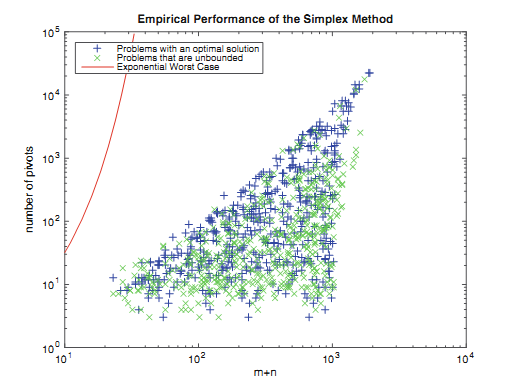
\includegraphics[scale=.5]{img/plot_1.png}
\caption{Đồ thị log-log thể hiện mối tương quan giữa $m$ + $n$ và số điểm xoay của bảng đơn hình (sample size = 1000)}
\end{figure}
\end{frame}

\begin{frame}[fragile]{Hiệu năng thực tế (cont.) - Kết quả thực nghiệm}
Dựa vào đồ thị, ta có được thông tin:
\begin{itemize}
\item \textcolor{red}{Đồ thị trên là đồ thị log-log}
\item Trong 1000 mẫu dữ liệu: có 501 mẫu trong dữ liệu có phương án tối ưu, trong khi 499 mẫu còn lại thì không có
\item Số lượng bài toán có $m$ > $n$ và $m$ < $n$ là xấp xỉ bằng nhau
\item Những bài toán có $m$ > $n$ gần như luôn có phương án tối ưu, và theo chiều ngược lại, $m$ < $n$ lại cho ta những bài toán nhiều khả năng là không có
\end{itemize}
\end{frame}

\begin{frame}[fragile]{Hiệu năng thực tế (cont.) - Kết quả thực nghiệm}
\begin{itemize}
\item Với mỗi giá trị $n$ + $m$, có vẻ như sẽ có 1 chặn trên cho số lượng phần tử xoay (giá trị trục tung)
\item Có rất nhiều bài toán được giải rất nhanh nhưng giá trị $n$ + $m$ lại lớn
\end{itemize}
$\rightarrow$ Có thể $n$ + $m$ không phải là một giá trị khảo sát tốt, ta sẽ thử 1 góc nhìn khác
\end{frame}

\begin{frame}[fragile]{Hiệu năng thực tế (cont.) - Kết quả thực nghiệm}
\begin{figure}
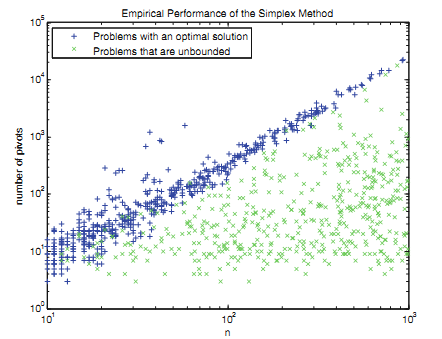
\includegraphics[scale=.5]{img/plot_2.png}
\caption{Đồ thị log-log với data y hệt đồ thị trước, nhưng thay đổi giá trị khảo sát trục hoành thành $n$}
\end{figure}
\end{frame}

\begin{frame}[fragile]{Hiệu năng thực tế (cont.) - Kết quả thực nghiệm}
Ta thu được nhận xét:
\begin{itemize}
\item Ở những điểm \textcolor{blue}{xanh dương}, là những bài toán có phương án tối ưu, ta thấy có sự tương quan rất rõ ràng hơn rất nhiều giữa độ lớn của $n$ với những điểm này
\item Ở những điểm \textcolor{codegreen}{xanh lục}, là những bài toán không có phương án tối ưu, ta nhận thấy chúng đều phân bố rời rạc,
\end{itemize}
\end{frame}

\begin{frame}[fragile]{Hiệu năng thực tế (cont.) - Kết quả thực nghiệm}
Dựa vào những thông tin này, ta dự đoán rằng, 1 bài toán "dễ" sẽ là bài toán sao cho $m$ hoặc $n$ sẽ nhỏ 1 cách tương đối với nhau \\
$\rightarrow$ Ta sẽ kiểm chứng bằng việc thử thay đổi giá trị khảo sát trục hoành thành $\min(m, n)$ \\
\end{frame}

\begin{frame}[fragile]{Hiệu năng thực tế (cont.) - Kết quả thực nghiệm}
\begin{figure}
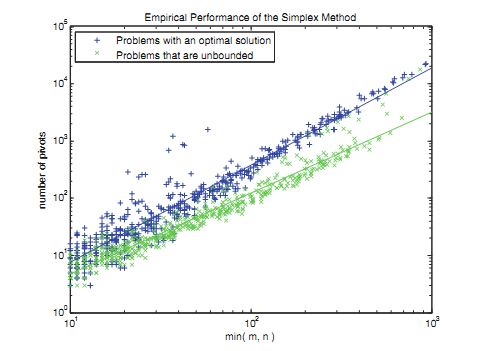
\includegraphics[scale=.5]{img/plot_3.png}
\caption{Đồ thị log-log với data y hệt 2 đồ thị trước, nhưng thay đổi giá trị khảo sát trục hoành thành $\min(m, n)$}
\end{figure}
\end{frame}

\begin{frame}[fragile]{Hiệu năng thực tế (cont.) - Kết quả thực nghiệm}
Hoàn hảo! Có vẻ như ta đã tìm được giá trị khảo sát tốt nhất cho cả 2 dạng bài toán \textcolor{blue}{có phương án tối ưu} và \textcolor{codegreen}{vô nghiệm}\\
Nhận xét: \textcolor{blue}{những điểm xanh dương} ở đồ thị này so với đồ thị trước, gần như không hề thay đổi vị trí\\
Giải thích: Vì phần lớn bài toán có phương án tối ưu sẽ có $n$ < $m$
\end{frame}

\begin{frame}[fragile]{Hiệu năng thực tế (cont.) - Kết quả thực nghiệm}
Sử dụng những kĩ thuật thống kê được đề cập ở Chương 12, ta có thể tìm được đường thẳng hồi quy cho đồ thị trên\\
Với những \textcolor{blue}{điểm xanh dương}, ta có được phương trình:
$$
log T \approx -1.90 + 1.70\log(\min(m, n))
$$
Với $T$ là số lần lặp (số điểm xoay) cần phải thực hiện để giải được 1 bài toán\\
Biến đổi phương trình, ta được:
$$
T \approx e^{-1.90}e^{1.70\log(min(m, n))} = 0.150min(m, n)^{1.70}
$$
\end{frame}

\begin{frame}[fragile]{Hiệu năng thực tế (cont.) - Kết quả thực nghiệm}
Tương tự với những \textcolor{codegreen}{điểm xanh lục}, ta có được phương trình:
$$
T \approx 0.180min(m, n)^{1.42}
$$
\end{frame}

\begin{frame}{Hiệu năng thực tế (cont.) - Kết quả thực nghiệm}
\begin{proof}[Kết luận thực nghiệm]
Số lần lặp (số phần tử xoay) trong một bài toán có phương án tối ưu  giải bằng phương pháp đơn hình là:
$$
\displaystyle
T \approx 0.150min(m, n)^{1.70}
$$
Số lần lặp (số phần tử xoay) trong một bài toán không có phương án tối ưu giải bằng phương pháp đơn hình là:
$$
\displaystyle
T \approx 0.180min(m, n)^{1.42}
$$
 
Với m là số ràng buộc và n là số biến
\end{proof}

Nhận xét: $T$ tăng so với $min(m, n)$ với tốc độ trên tuyến tính (superlinear)

\end{frame}

\begin{frame}[fragile]{Hiệu năng thực tế (cont.) - Kết quả thực nghiệm}
\begin{figure}
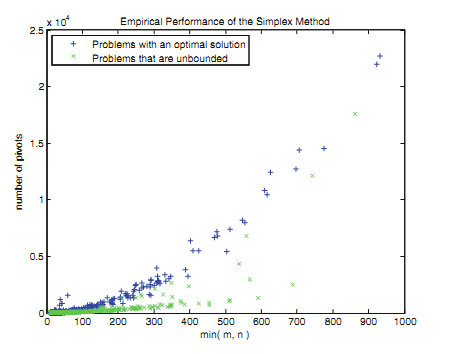
\includegraphics[scale=.5]{img/plot_4.png}
\caption{Đồ thị với data y hệt 3 đồ thị trước, nhưng không sử dụng đồ thị dạng log-log để thể hiện tốc độ tăng trên tuyến tính của số phần tử xoay}
\end{figure}
\end{frame}

\section{Tài liệu tham khảo}
\begin{frame}[allowframebreaks]{Tài liệu tham khảo}
\printbibliography
\end{frame}
\end{document}
